%%%%%%%%%%%%%%%%%%%%%%%%%%%%%%%%%%%%%%%%%%%%%%%%%%%%%%%%%%%%%%%%%%%%%%%%%%%%%%%%%%%%%%%%%%%%%%%%%%%%%%%%%%%%%%%%%%%%%%%%%%%%%%%%%%%%%%%%%%%%%%%%%%%%%%%%%%%
% This is just an example/guide for you to refer to when producing your supplementary material for your Frontiers article.                                 %
%%%%%%%%%%%%%%%%%%%%%%%%%%%%%%%%%%%%%%%%%%%%%%%%%%%%%%%%%%%%%%%%%%%%%%%%%%%%%%%%%%%%%%%%%%%%%%%%%%%%%%%%%%%%%%%%%%%%%%%%%%%%%%%%%%%%%%%%%%%%%%%%%%%%%%%%%%%

%%% Version 2.5 Generated 2018/06/15 %%%
%%% You will need to have the following packages installed: datetime, fmtcount, etoolbox, fcprefix, which are normally inlcuded in WinEdt. %%%
%%% In http://www.ctan.org/ you can find the packages and how to install them, if necessary. %%%
%%%  NB logo1.jpg is required in the path in order to correctly compile front page header %%%

\documentclass[utf8]{frontiers_suppmat} % for all articles
\usepackage{url,hyperref,lineno,microtype}
\usepackage[onehalfspacing]{setspace}



% Leave a blank line between paragraphs instead of using \\

\begin{document}
\onecolumn
\firstpage{1}

\title {{\helveticaitalic{Supplementary Material}}}


\maketitle


\section{Summary}

We have provided supplementary material to our article titled ``Computational aspects of the equivalent-layer technique: review''.
In this accompanying material, we present five additional synthetic data results with the equivalent layer estimated by using different 
methods.

\section{Supplementary results with synthetic data}


In the main paper, the subsection 8.3 ``Stability analysis and gravity-gradient components''
shows the results of the equivalent-layer technique using the iterative deconvolution, 
proposed by \cite{takahashi-etal2020}, for processing gravity-gradient data.

In this accompanying material, we inverted the same noise-corrupted gravity disturbance presented in the main paper.
Here, the gravity-gradient data (not shown) were predicted by the equivalent layer (not shown) estimated by using the following methods:
\begin{itemize}
	\item[i)] CGLS;
	\item[ii)] Cholesky factorization;
	\item[iii)] iterative method proposed by \citet{siqueira-etal2017};
	\item[iv)] direct deconvolution with optimal value of $\zeta = 10^{-22}$; and
	\item[v)] column-action proposed by \cite{cordell1992}.
\end{itemize}
The algorithms for these methods are outlined in the main manuscript.

By using CGLS method, Figures \ref{fig:residuals-CGLS}\textbf{(A)}--\textbf{(F)} show the residuals (in Eötvös) 
between the predicted (not shown) and noise-free gravity-gradient data 
and Figure \ref{fig:residuals-CGLS}\textbf{(G)} shows the residuals (in mGal) between the predicted and noise-corrupted gravity disturbances.

By using Cholesky factorization, Figures\ref{fig:residuals-Cholesky}\textbf{(A)}--\textbf{(F)} 
show the residuals (in Eötvös) between the predicted (not shown) and noise-free gravity-gradient data 
and Figure \ref{fig:residuals-Cholesky}\textbf{(G)} shows the residuals (in mGal) between the predicted and noise-corrupted gravity disturbances.

By using the iterative method proposed by \citet{siqueira-etal2017}, 
Figures \ref{fig:residuals-SOB17}\textbf{(A)}--\textbf{(F)}  show  the residuals (in Eötvös) between the predicted (not shown) and 
noise-free gravity-gradient data and Figure \ref{fig:residuals-SOB17}\textbf{(G)} shows the residuals (in mGal) between the predicted 
and noise-corrupted gravity disturbances.

Figures \ref{fig:residuals-CGLS}, \ref{fig:residuals-Cholesky}  and \ref{fig:residuals-SOB17} 
show that the CGLS method, the Cholesky factorization, the iterative method proposed by 
\citet{siqueira-etal2017} yield acceptable data fittings despite their 
significant difference in floating-point operations. 

By using direct deconvolution with optimal value of $\zeta = 10^{-22}$, 
Figures \ref{fig:residuals-deconv} \textbf{(A)}--\textbf{(F)} show the residuals (in Eötvös) between 
the predicted (not shown) and noise-free gravity-gradient data and Figure \ref{fig:residuals-deconv}\textbf{(G)} shows the residuals (in mGal) between the predicted and noise-corrupted gravity disturbances.


By using the iterative method  proposed by \cite{cordell1992}, 
Figures \ref{fig:residuals-C92}\textbf{(A)}--\textbf{(F)}  show  the residuals (in Eötvös) between the predicted 
(not shown) and noise-free gravity-gradient data and Figure \ref{fig:residuals-C92}\textbf{(G)} 
shows the residuals (in mGal) between the predicted and noise-corrupted gravity disturbances.

Due to the border effects, the residuals from the direct deconvolution 
(Figure \ref{fig:residuals-deconv}) are greater than those predicted using 
CGLS method, Cholesky factorization and the iterative method proposed 
by \citet{siqueira-etal2017} (Figures \ref{fig:residuals-CGLS}, 
\ref{fig:residuals-Cholesky}  and \ref{fig:residuals-SOB17}).
Finally, we stress that the iterative method  proposed by \cite{cordell1992}  produces 
the worst fit data fit. The main difficulty with this method is setting the depth of the
equivalent sources for each datum.

%\section{Supplementary Data}
%
%Supplementary Material should be uploaded separately on submission. Please include any supplementary data, figures and/or tables. All supplementary files are deposited to FigShare for permanent storage and receive a DOI.
%
%Supplementary material is not typeset so please ensure that all information is clearly presented, the appropriate caption is included in the file and not in the manuscript, and that the style conforms to the rest of the article. To avoid discrepancies between the published article and the supplementary material, please do not add the title, author list, affiliations or correspondence in the supplementary files.
%
%\section{Supplementary Tables and Figures}
%
%For more information on Supplementary Material and for details on the different file types accepted, please see \href{https://www.frontiersin.org/about/author-guidelines#supplementary-material}{the Supplementary Material section} of the Author Guidelines.
%
%Figures, tables, and images will be published under a Creative Commons CC-BY licence and permission must be obtained for use of copyrighted material from other sources (including re-published/adapted/modified/partial figures and images from the internet). It is the responsibility of the authors to acquire the licenses, to follow any citation instructions requested by third-party rights holders, and cover any supplementary charges.

%% Figures, tables, and images will be published under a Creative Commons CC-BY licence and permission must be obtained for use of copyrighted material from other sources (including re-published/adapted/modified/partial figures and images from the internet). It is the responsibility of the authors to acquire the licenses, to follow any citation instructions requested by third-party rights holders, and cover any supplementary charges.

\bibliographystyle{Frontiers-Harvard}
%\bibliographystyle{frontiersinSCNS_ENG_HUMS} %  for Science, Engineering and Humanities and Social Sciences articles, for Humanities and Social Sciences articles please include page numbers in the in-text citations
%\bibliographystyle{frontiersinHLTH&FPHY} % for Health and Physics articles
\bibliography{references_supp}

\section{Supplementary figures}

\begin{figure}[htbp]
	\begin{center}
		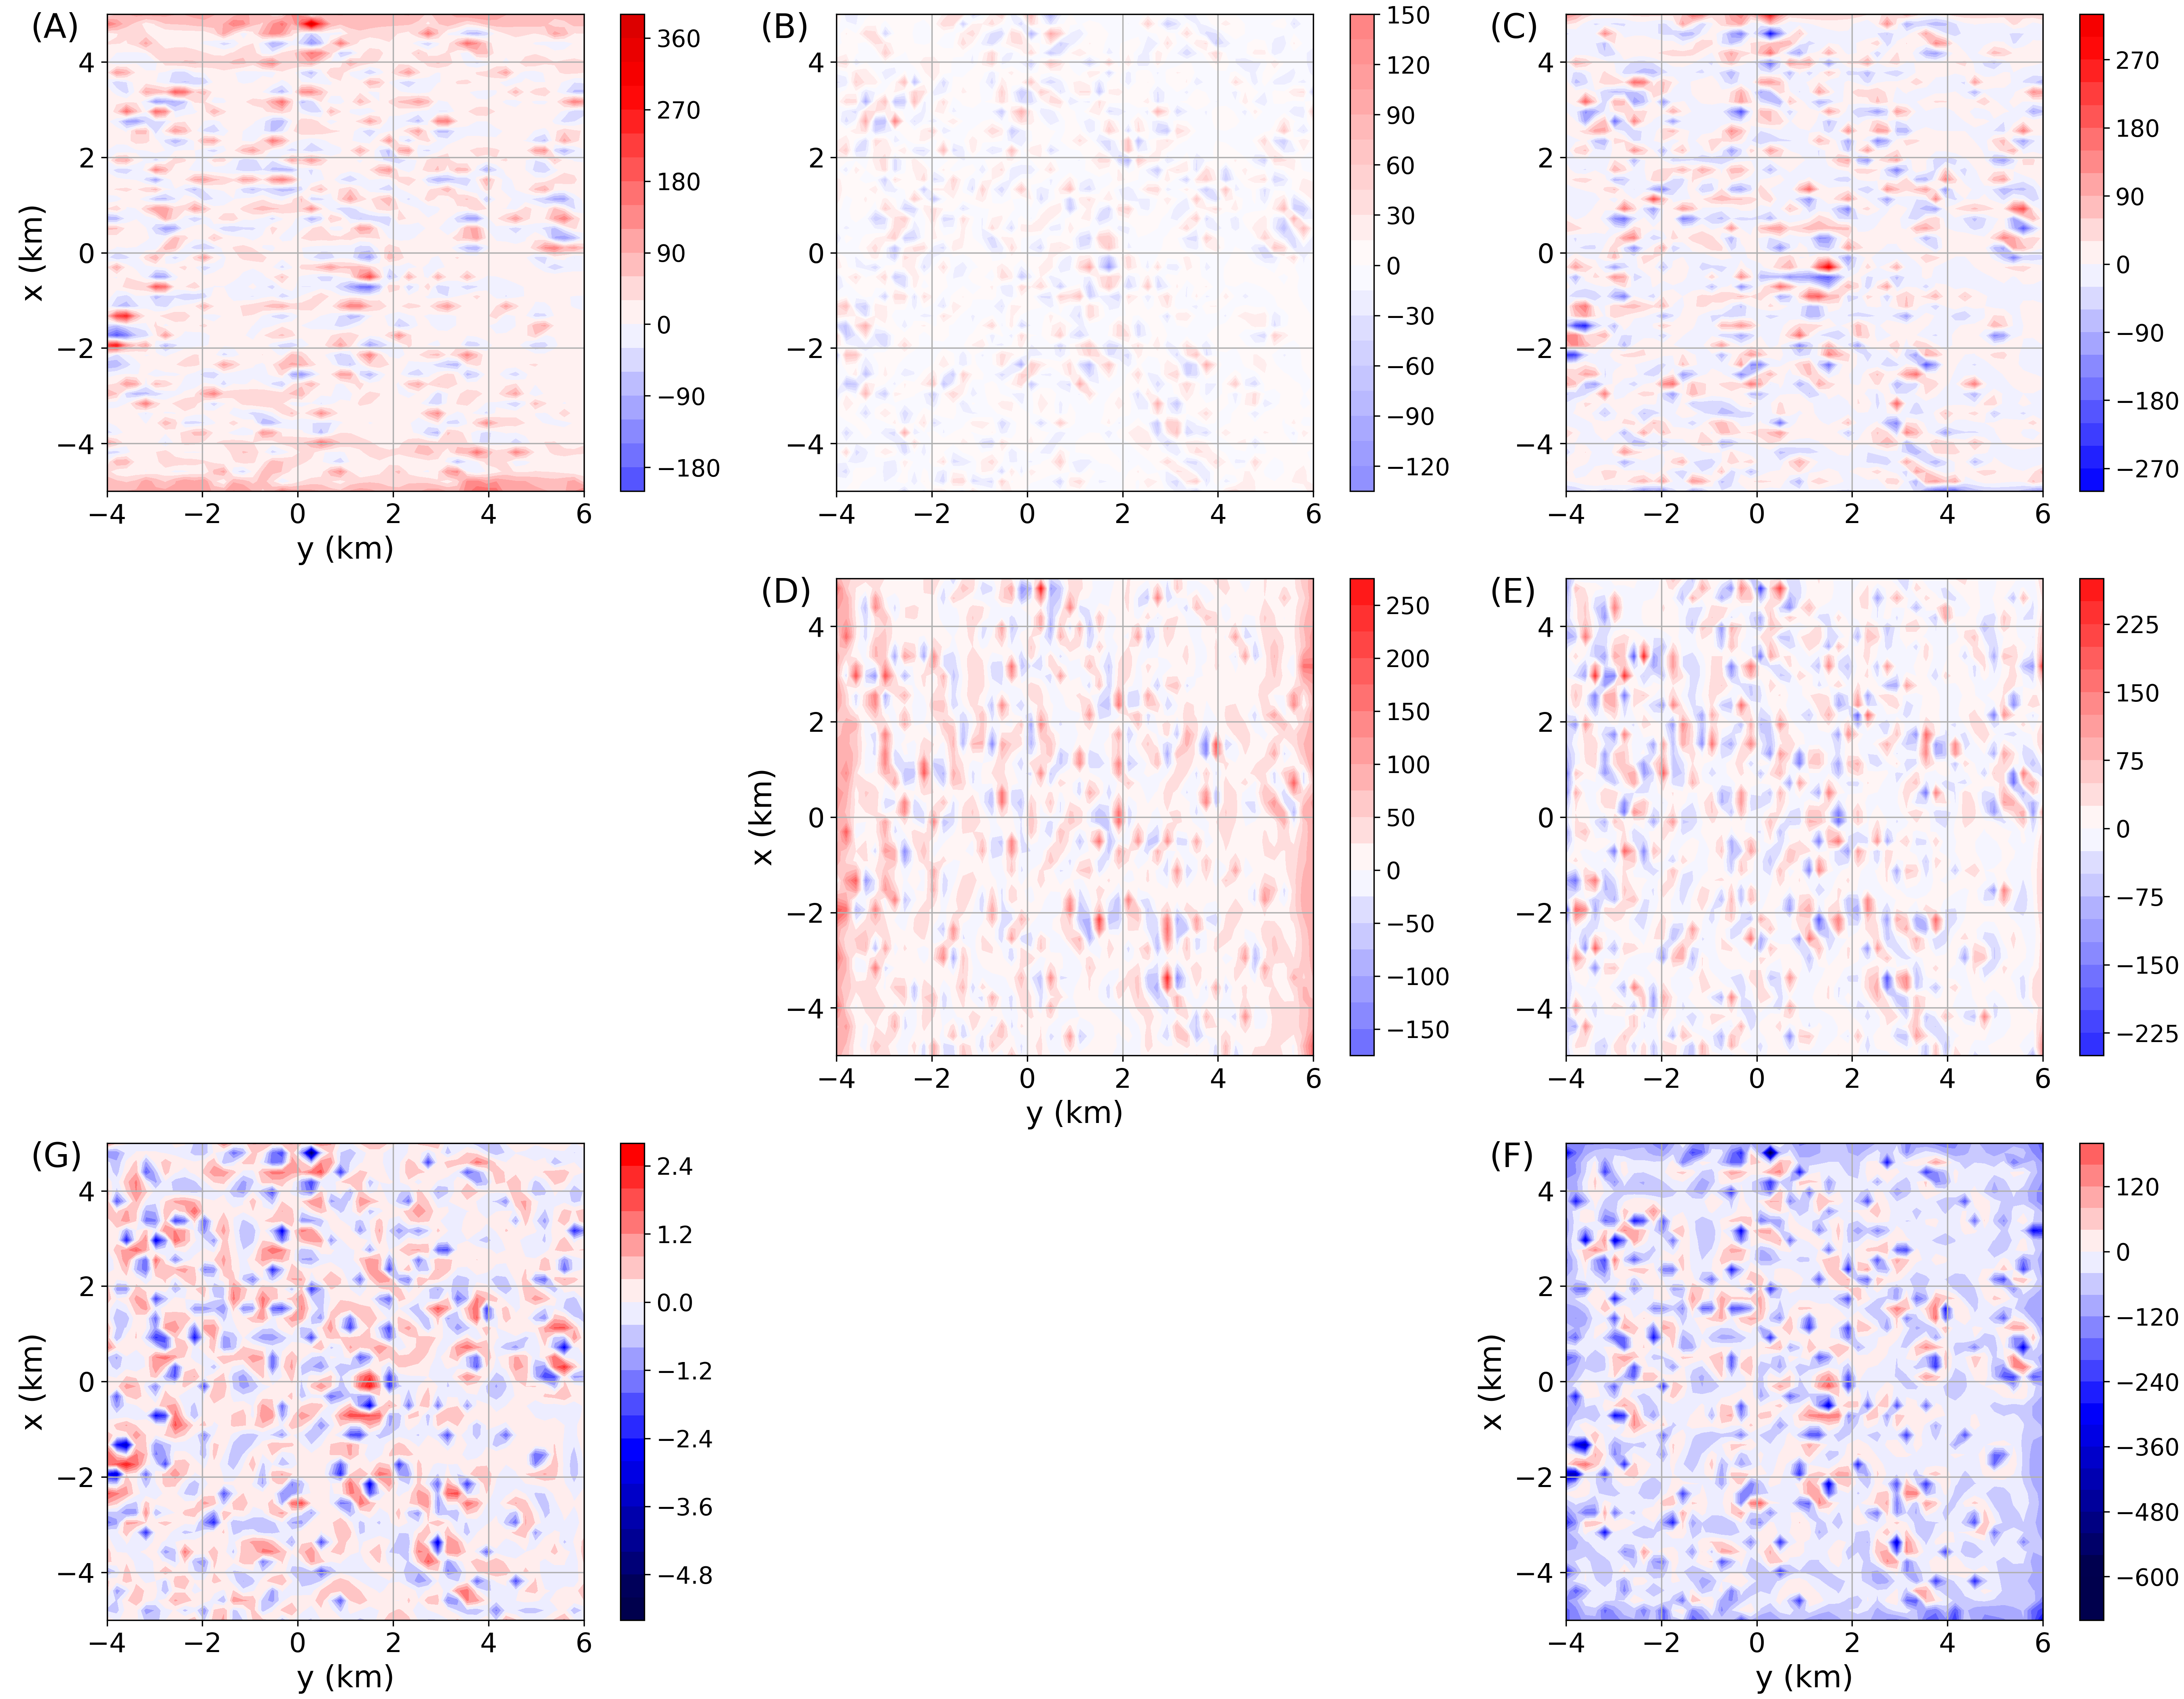
\includegraphics[width=10cm]{Fig/CGLS_residuals}
	\end{center}
	\caption{
		Residuals between the gravity data predicted by the equivalent layer estimated with 
		the CGLS method.
		The inverse problems was solved by using the noise-corrupted gravity 
		disturbance having the maximum noise level (not shown).
		Panels \textbf{(A)}--\textbf{(F)} show the residuals between the predicted and 
		noise-free gravity gradient data. The values are in Eötvös.
		\textbf{(G)} Shows the residuals between the predicted and noise-corrupted gravity 
		disturbances. The values are in milligals (mGal).
	}
	\label{fig:residuals-CGLS}
\end{figure}

\begin{figure}[htbp]
	\begin{center}
		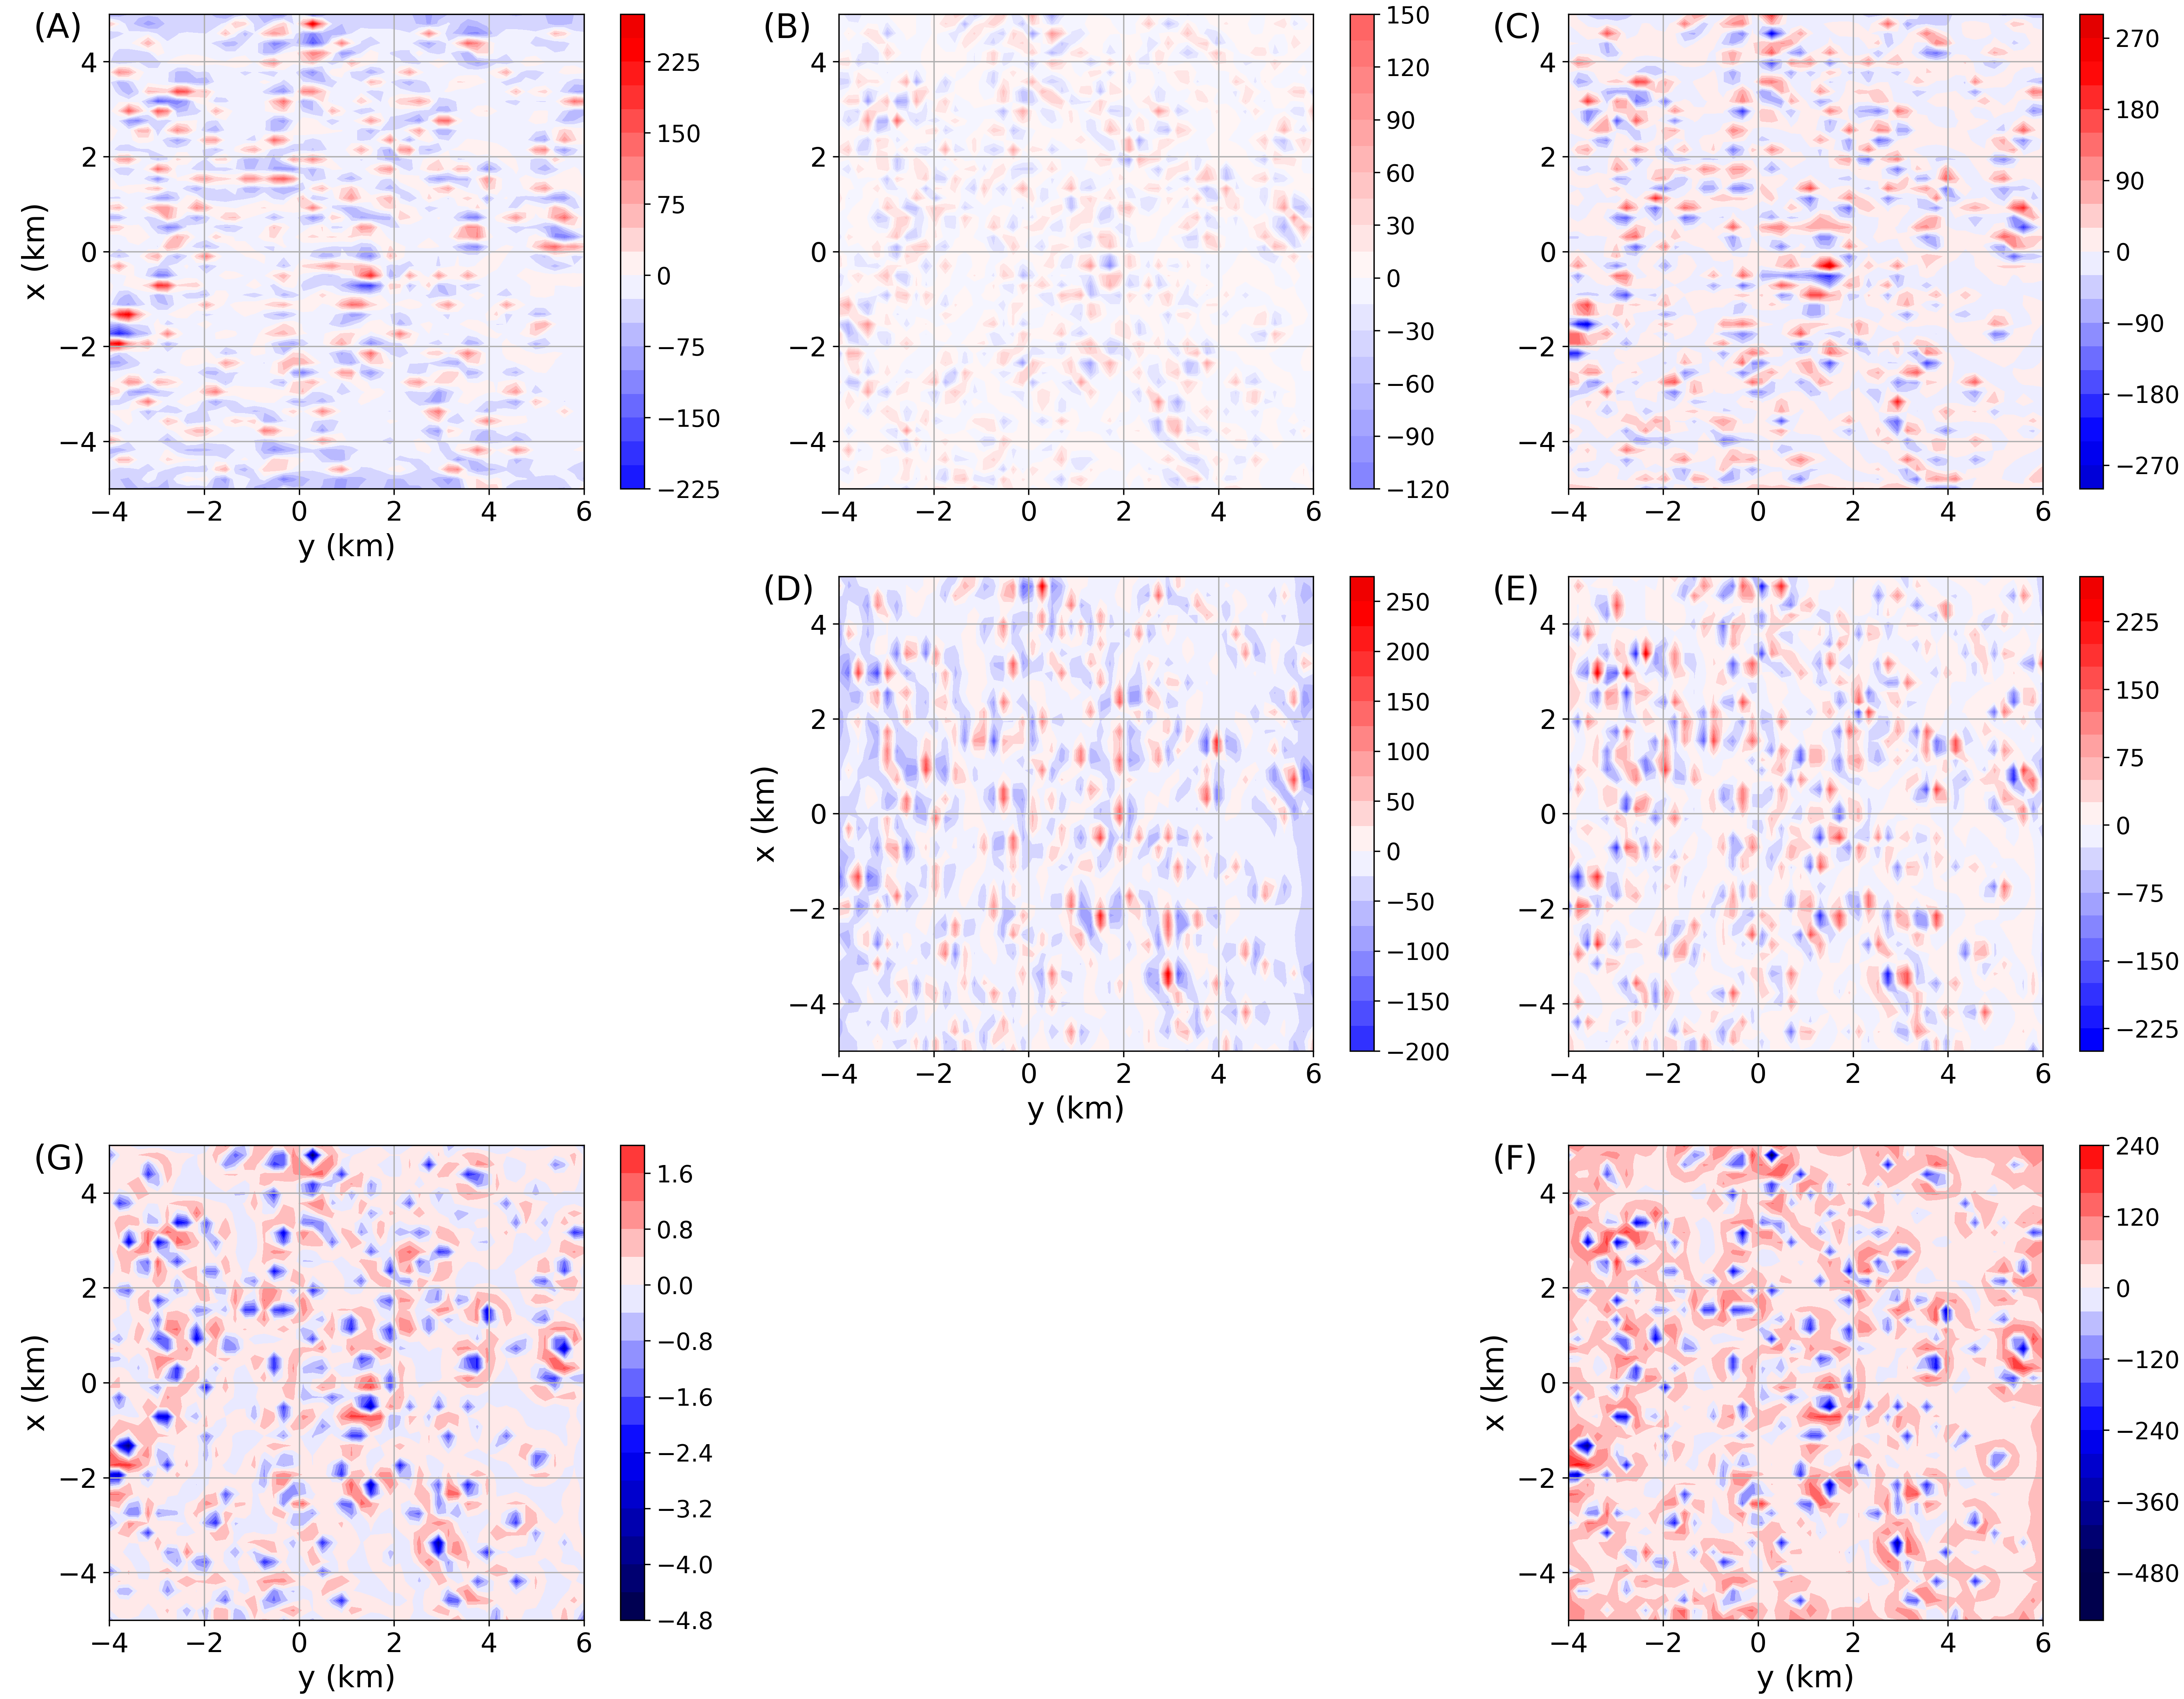
\includegraphics[width=10cm]{Fig/Cholesky_residuals}
	\end{center}
	\caption{
		Residuals between the gravity data predicted by the equivalent layer estimated with 
		the Cholesky factorization.
		The inverse problems was solved by using the noise-corrupted gravity 
		disturbance having the maximum noise level (not shown).
		Panels \textbf{(A)}--\textbf{(F)} show the residuals between the predicted and 
		noise-free gravity gradient data. The values are in Eötvös.
		\textbf{(G)} Shows the residuals between the predicted and noise-corrupted gravity 
		disturbances. The values are in milligals (mGal).
	}
	\label{fig:residuals-Cholesky}
\end{figure}

\begin{figure}[htbp]
	\begin{center}
		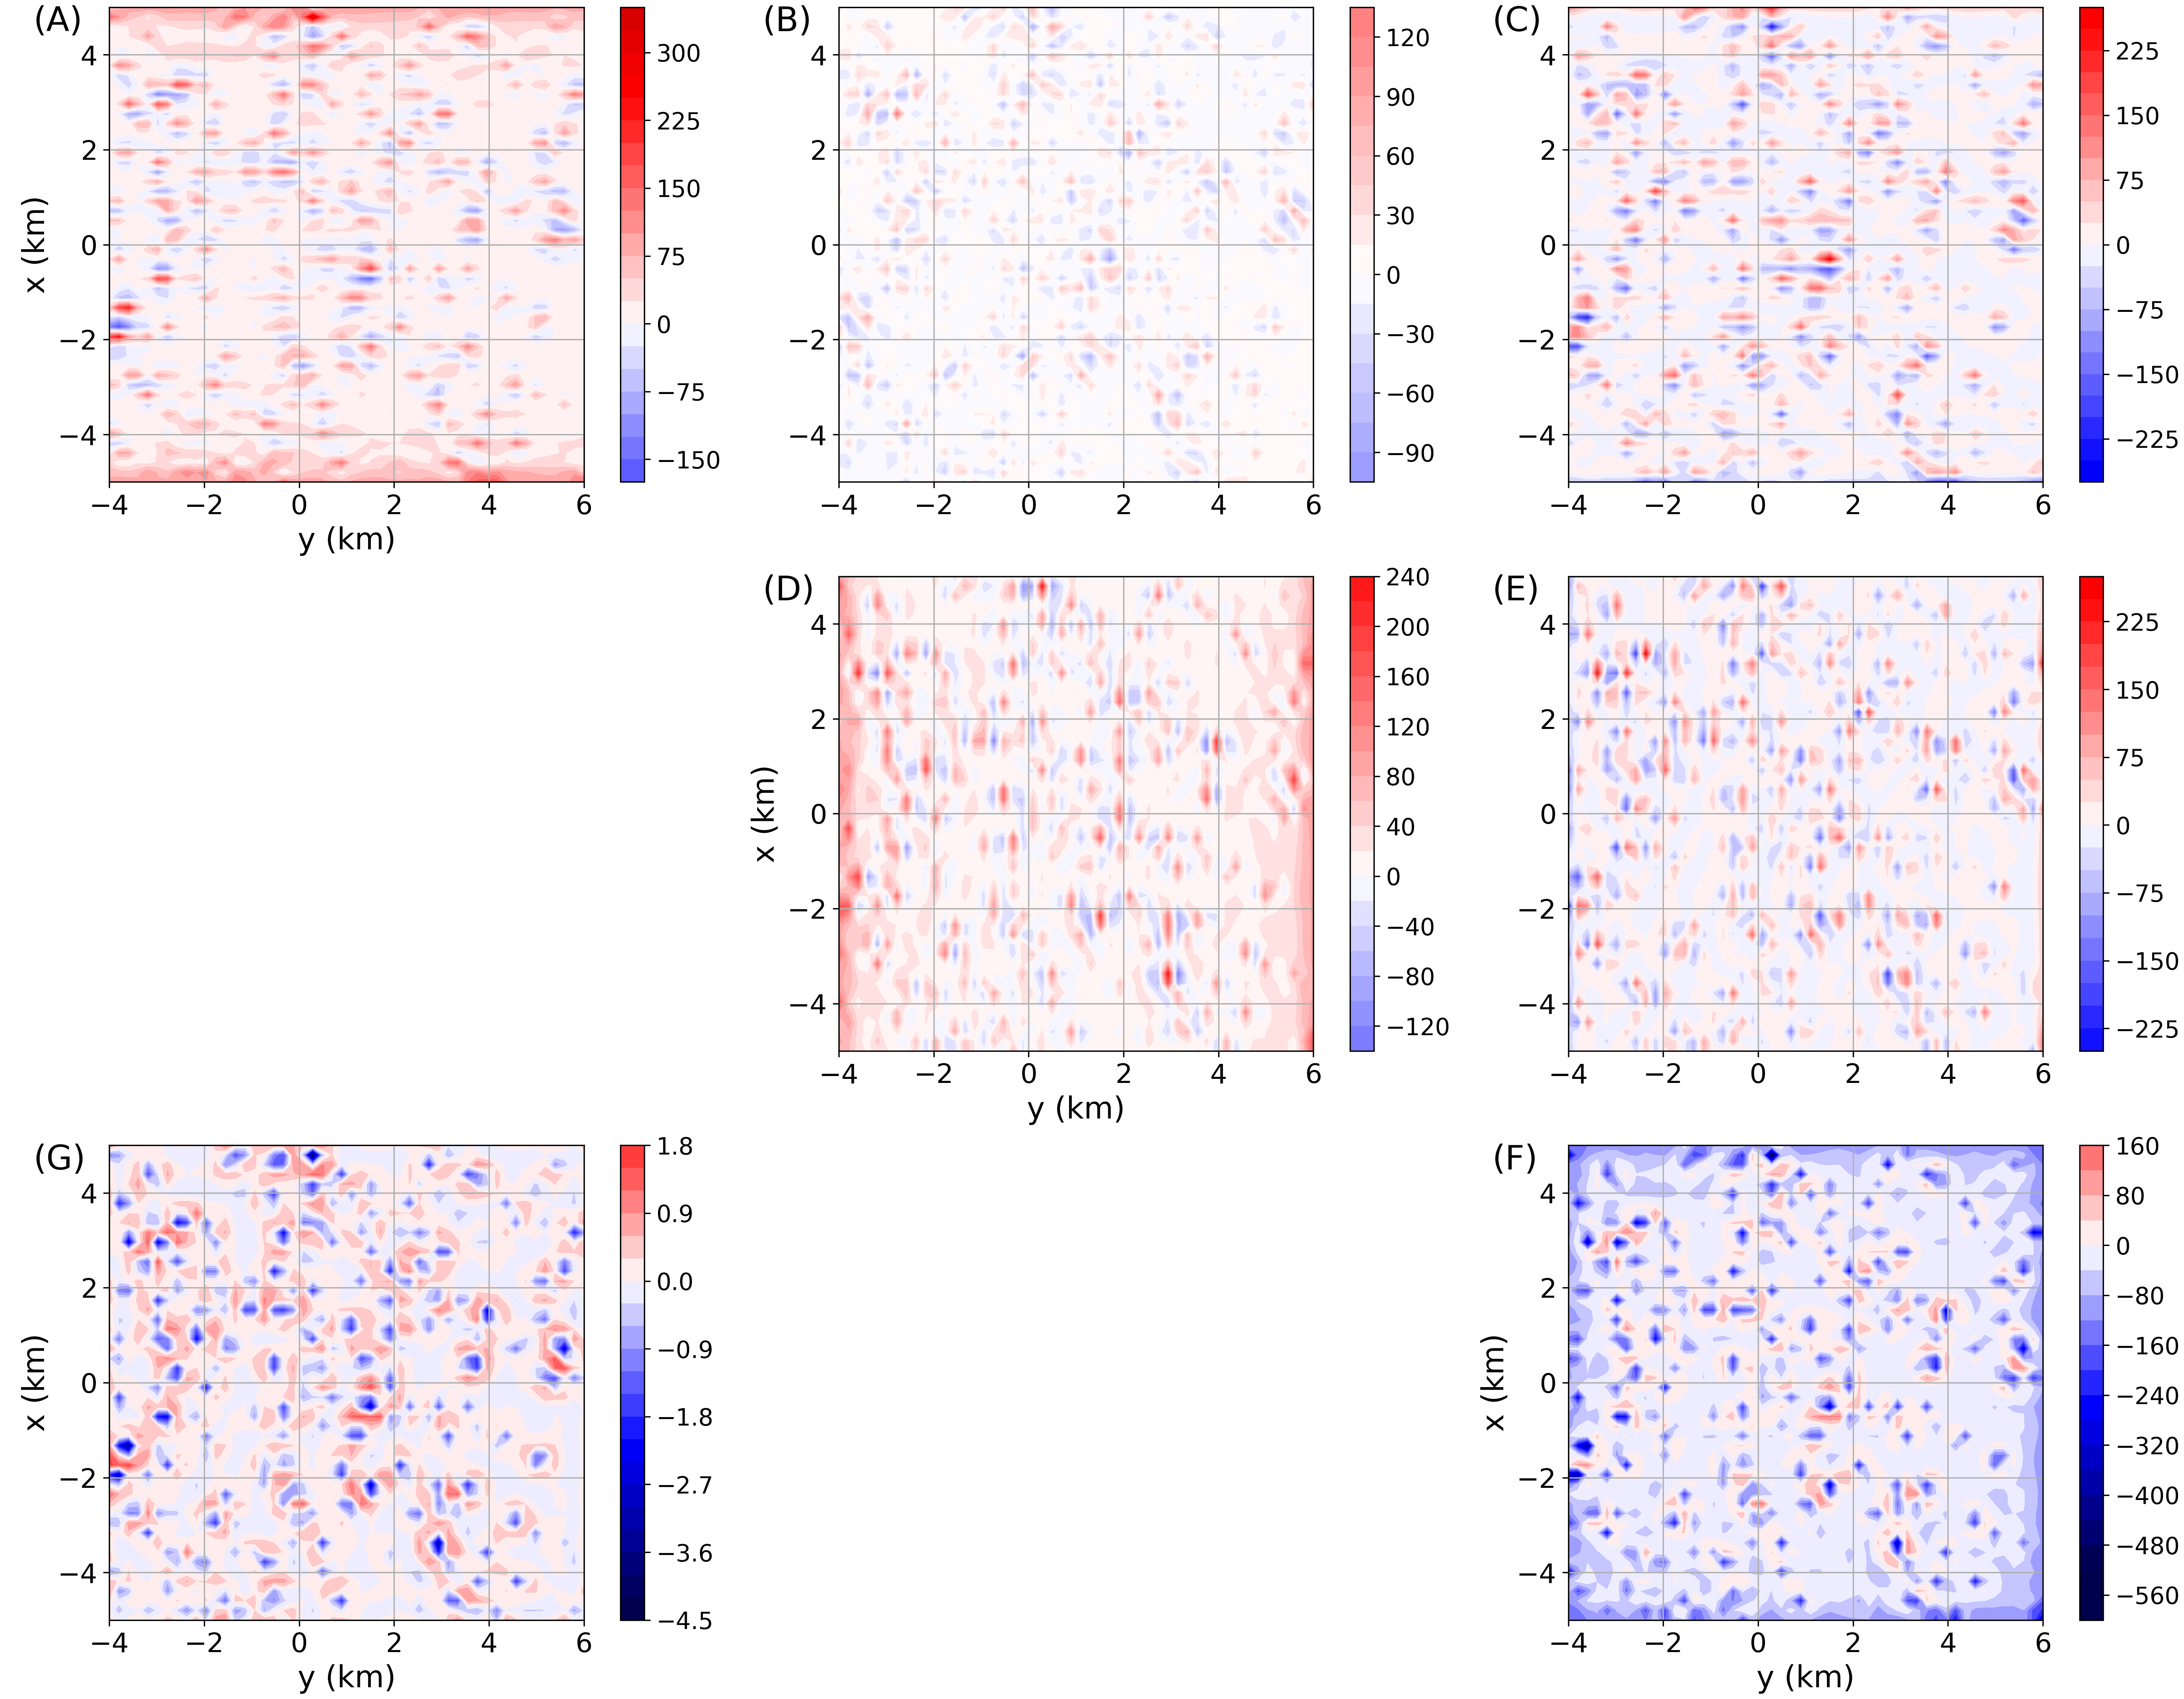
\includegraphics[width=10cm]{Fig/SOB17_residuals}
	\end{center}
	\caption{
		Residuals between the gravity data predicted by the equivalent layer estimated with 
		the iterative method proposed by \citet{siqueira-etal2017}.
		The inverse problems was solved by using the noise-corrupted gravity 
		disturbance having the maximum noise level (not shown).
		Panels \textbf{(A)}--\textbf{(F)} show the residuals between the predicted and 
		noise-free gravity gradient data. The values are in Eötvös.
		\textbf{(G)} Shows the residuals between the predicted and noise-corrupted gravity 
		disturbances. The values are in milligals (mGal).
	}
	\label{fig:residuals-SOB17}
\end{figure}

\begin{figure}[htbp]
	\begin{center}
		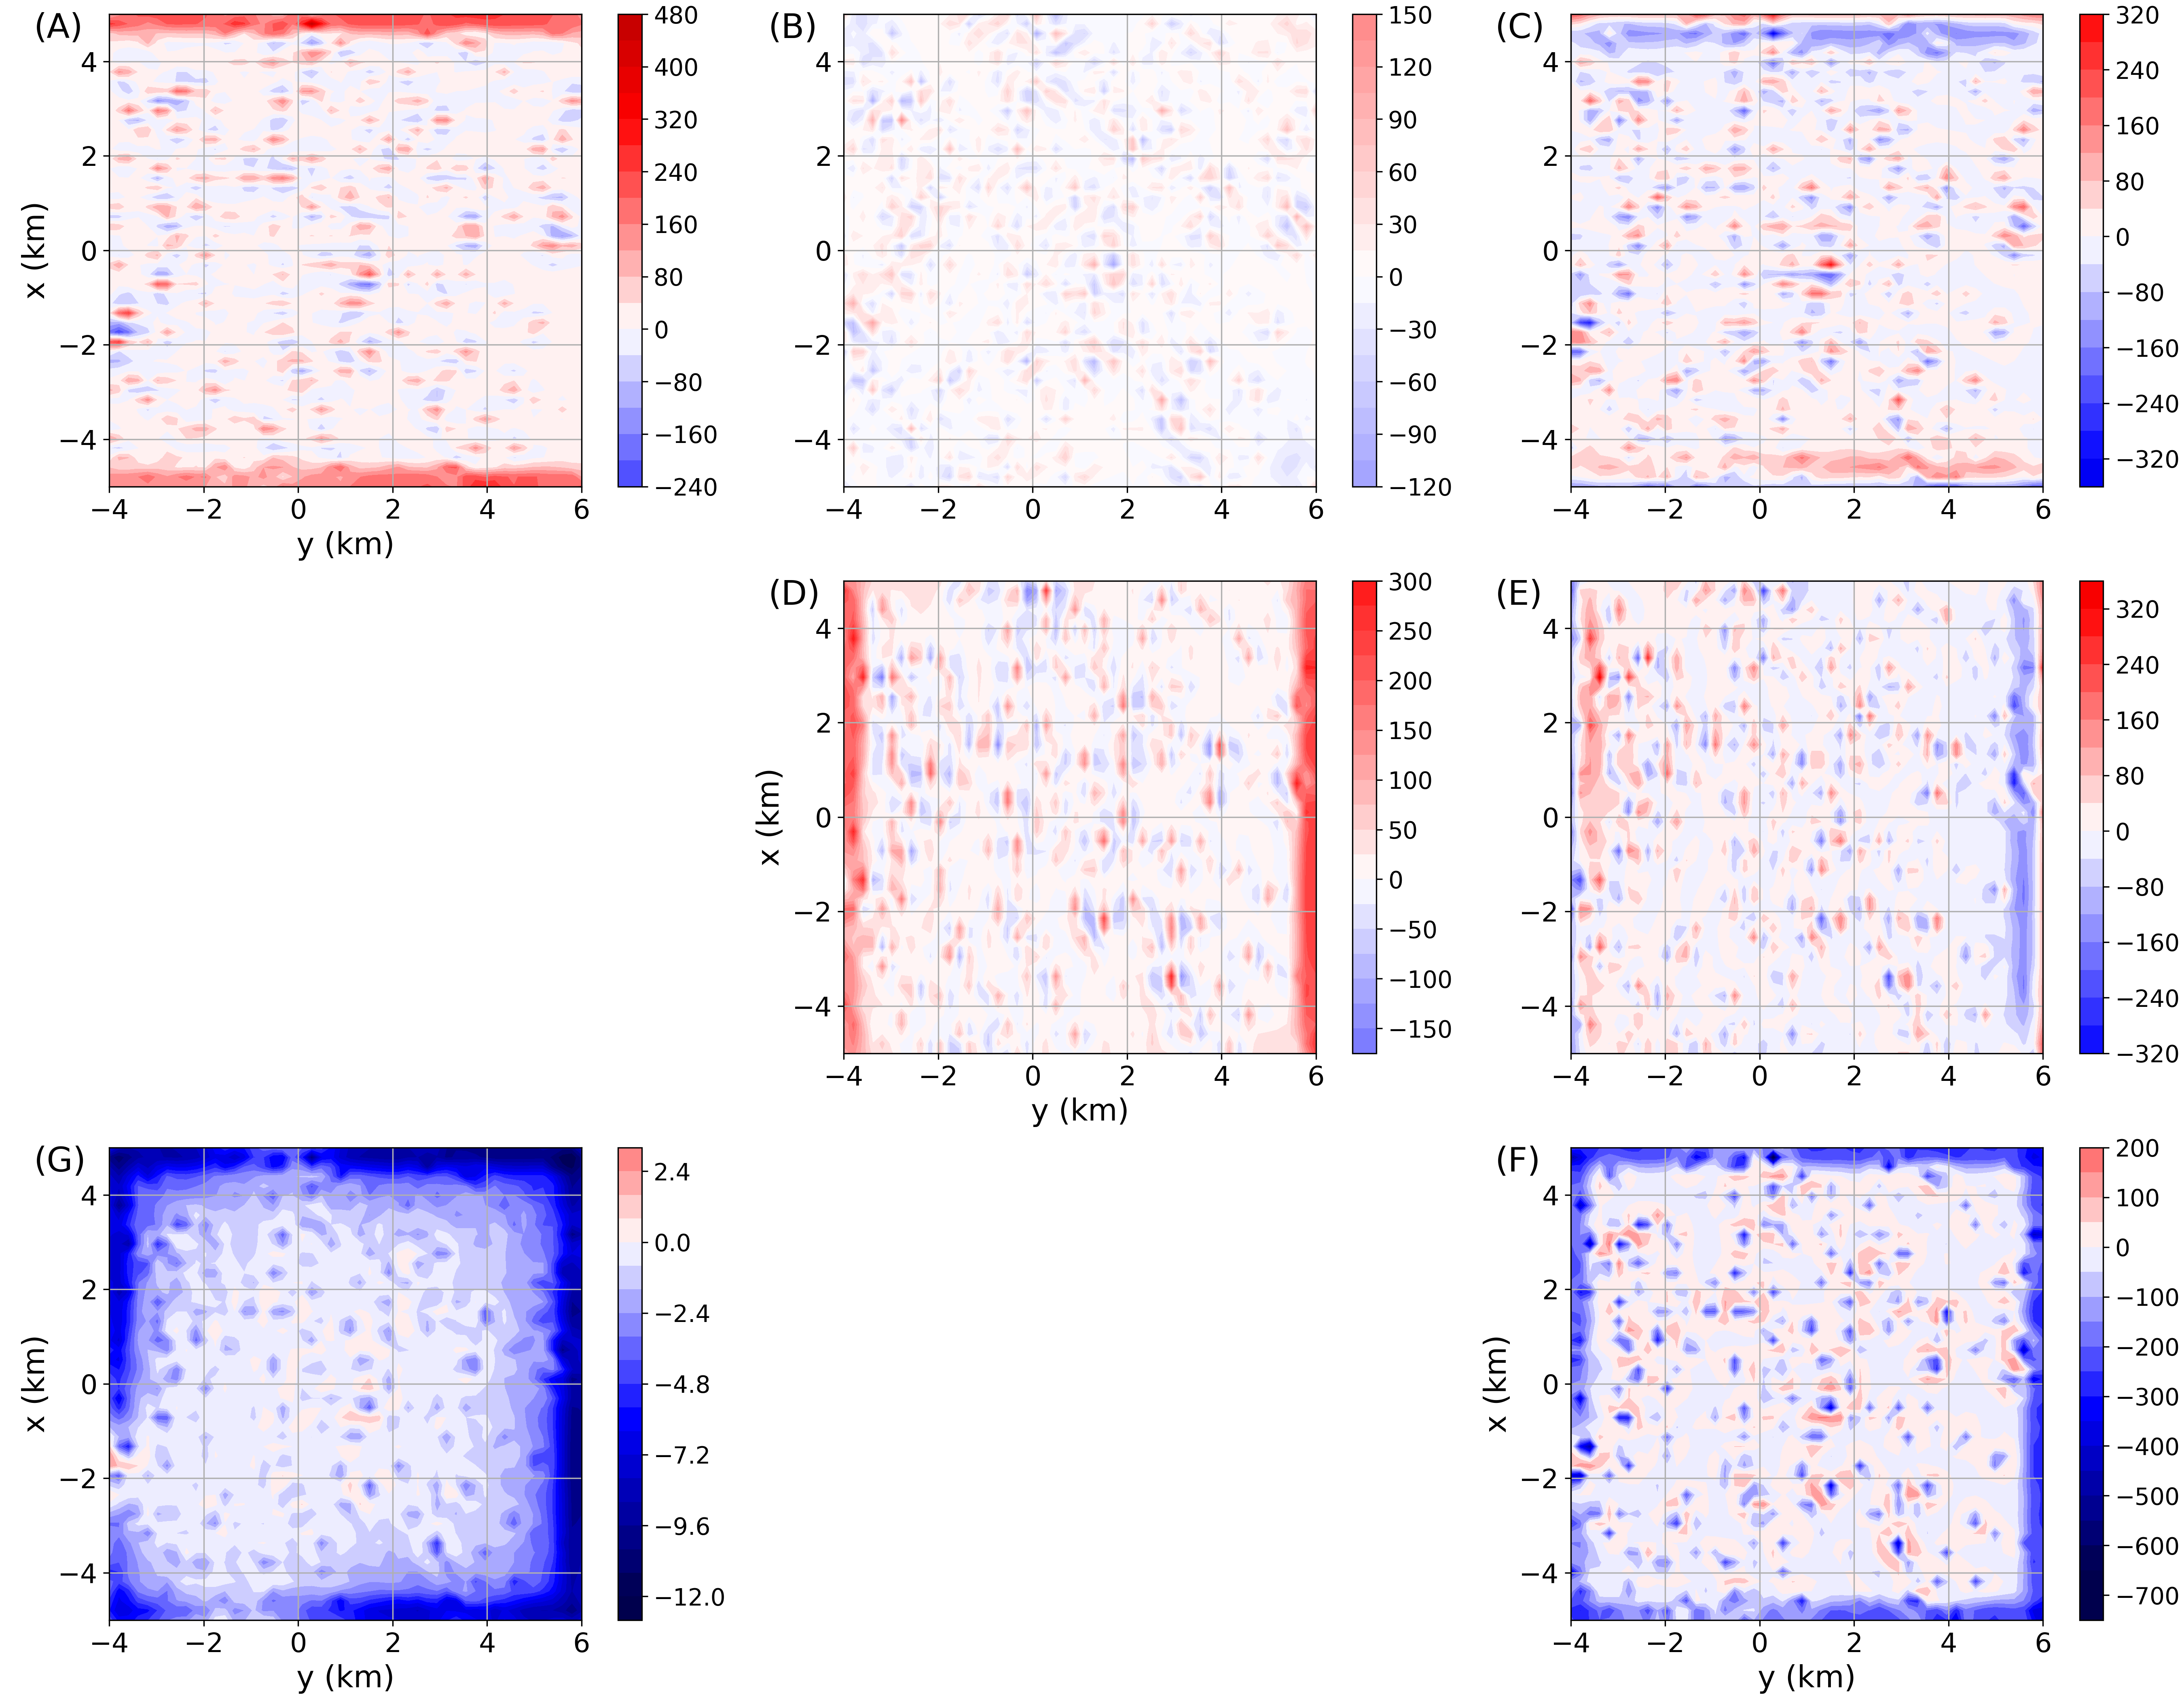
\includegraphics[width=10cm]{Fig/deconv_residuals}
	\end{center}
	\caption{
		Residuals between the gravity data predicted by the equivalent layer estimated with 
		the direct deconvolution with  optimal value of $\zeta = 10^{-22}$.
		The inverse problems was solved by using the noise-corrupted gravity 
		disturbance having the maximum noise level (not shown).
		Panels \textbf{(A)}--\textbf{(F)} show the residuals between the predicted and 
		noise-free gravity gradient data. The values are in Eötvös.
		\textbf{(G)} Shows the residuals between the predicted and noise-corrupted gravity 
		disturbances. The values are in milligals (mGal).
	}
	\label{fig:residuals-deconv}
\end{figure}
	
\begin{figure}[htbp]
	\begin{center}
		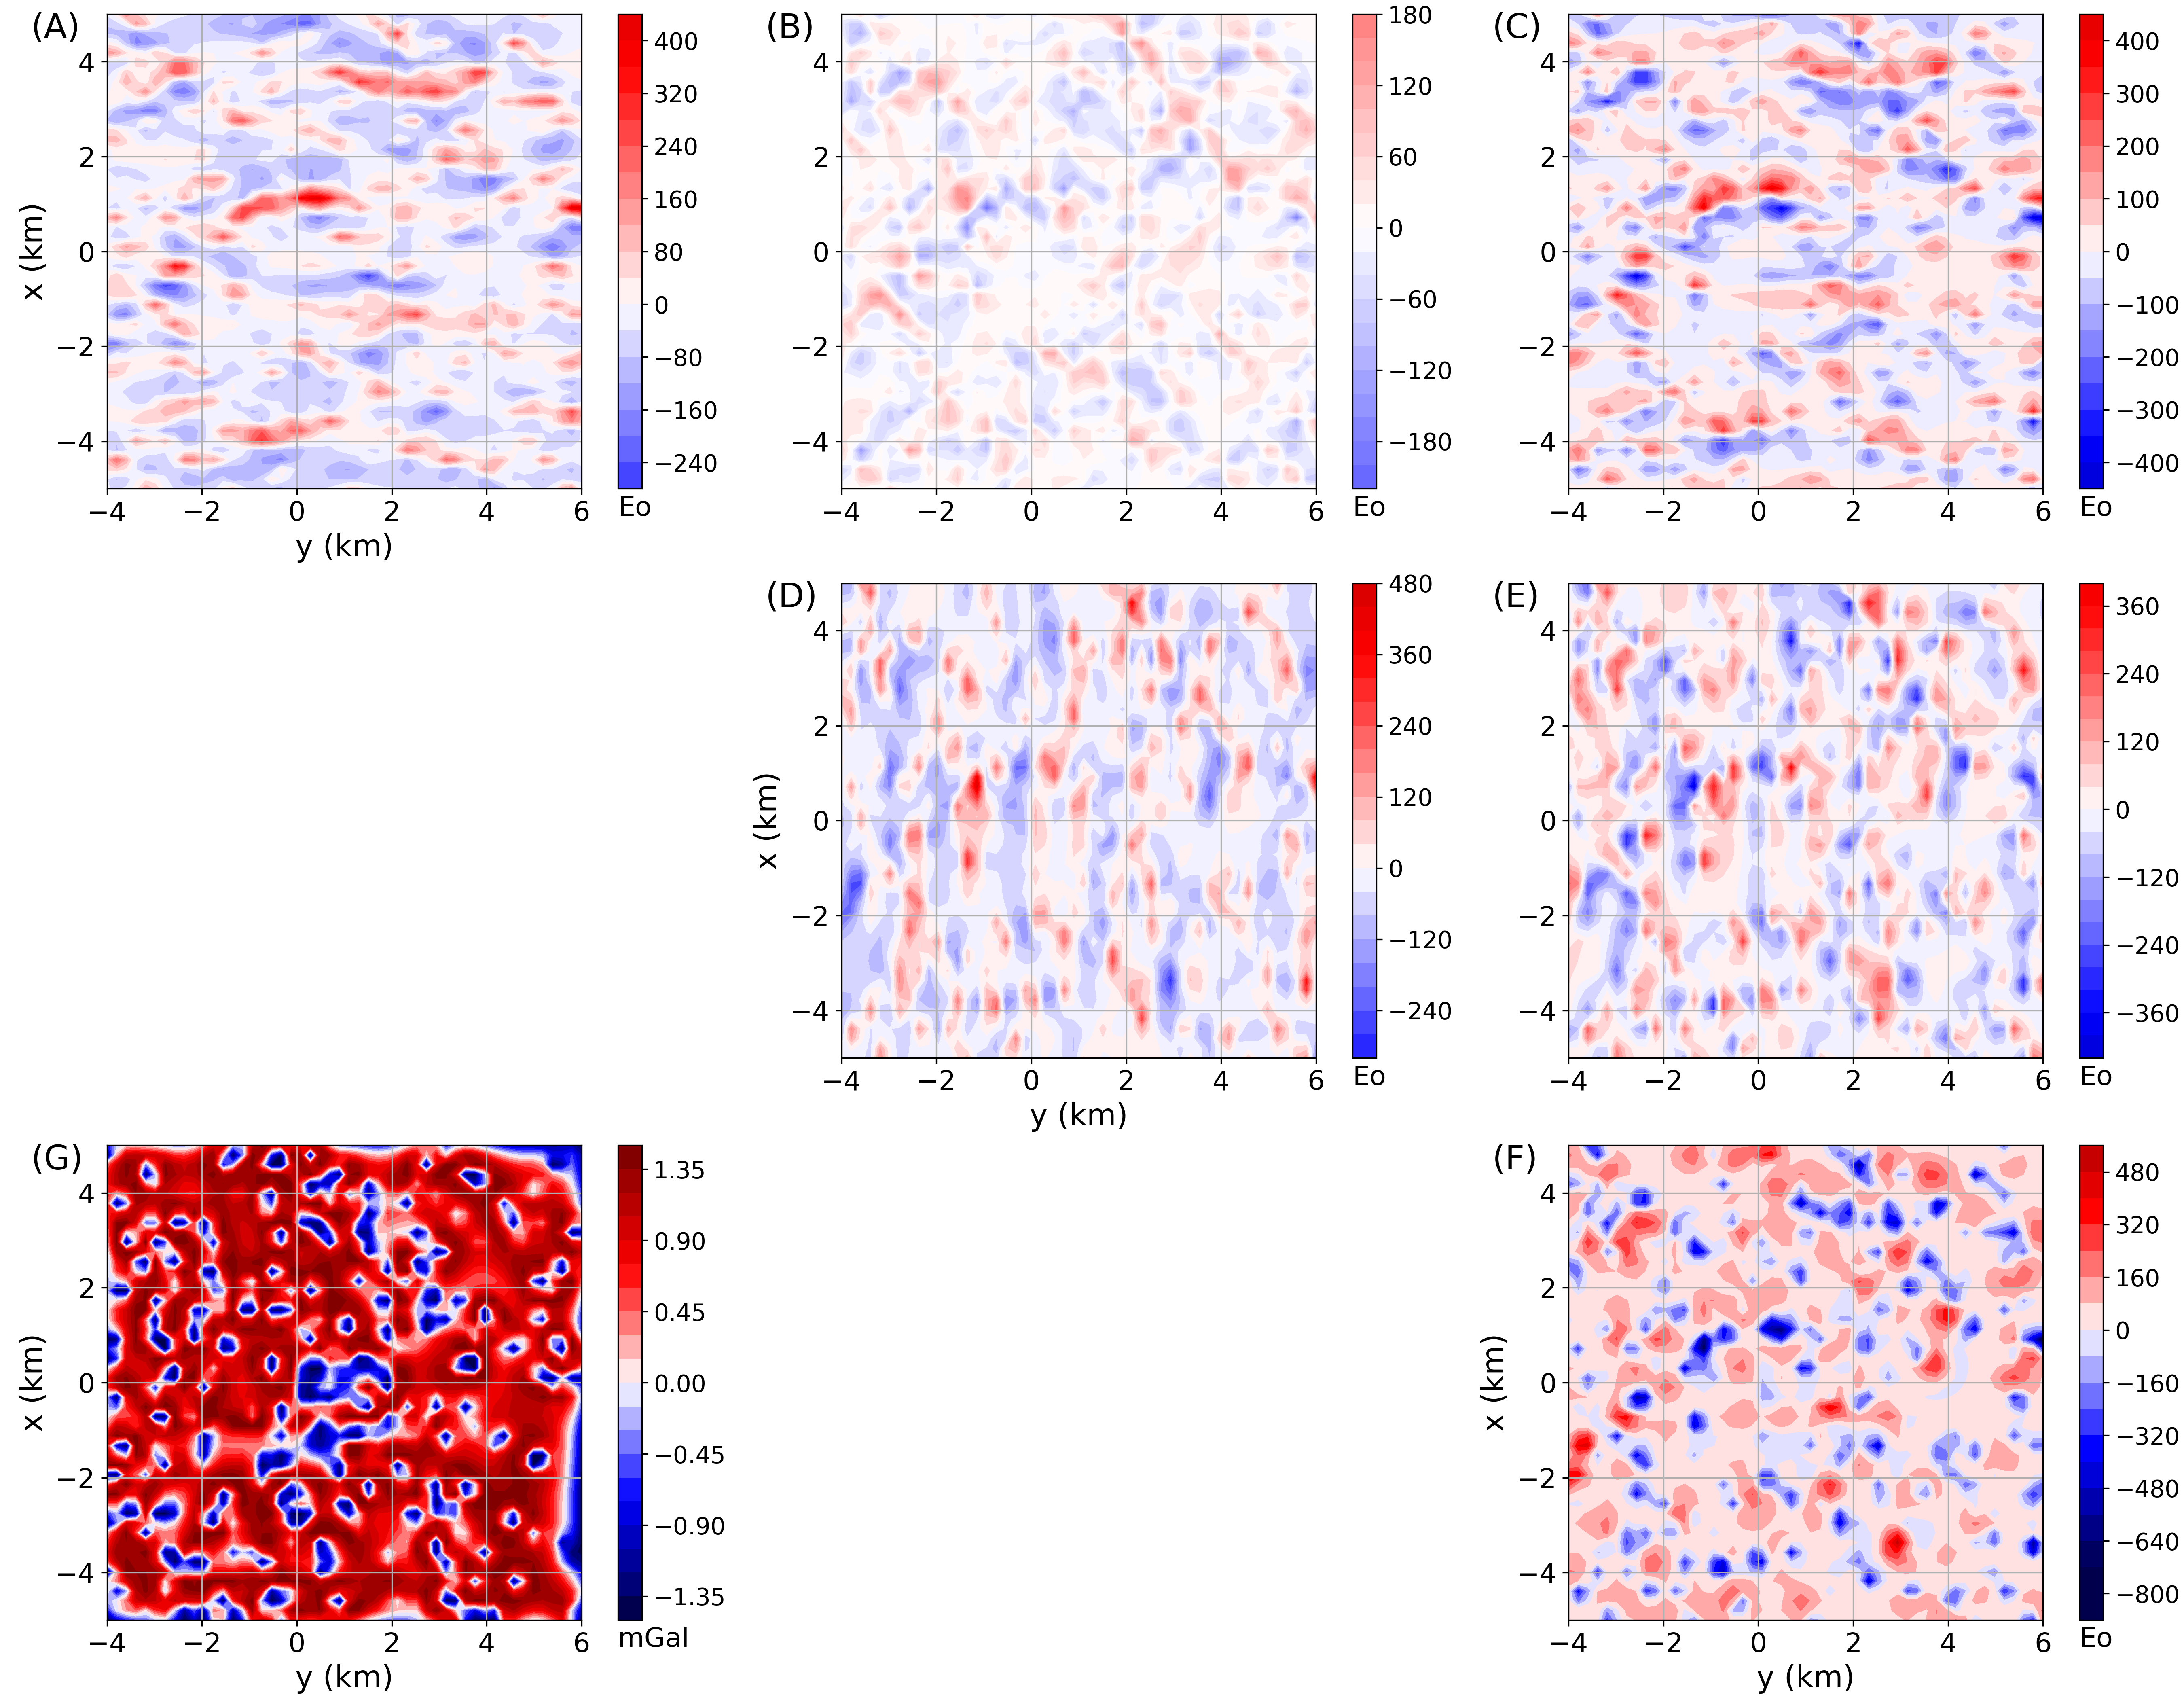
\includegraphics[width=10cm]{Fig/C92_residuals}
	\end{center}
	\caption{
		Residuals between the gravity data predicted by the equivalent layer estimated with 
		the iterative method  proposed by \cite{cordell1992}.
		The inverse problems was solved by using the noise-corrupted gravity 
		disturbance having the maximum noise level (not shown).
		Panels \textbf{(A)}--\textbf{(F)} show the residuals between the predicted and 
		noise-free gravity gradient data. The values are in Eötvös.
		\textbf{(G)} Shows the residuals between the predicted and noise-corrupted gravity 
		disturbances. The values are in milligals (mGal).
	}
	\label{fig:residuals-C92}
\end{figure}

%%% There is no need for adding the file termination, as long as you indicate where the file is saved. In the examples below the files (logo1.eps and logos.eps) are in the Frontiers LaTeX folder
%%% If using *.tif files convert them to .jpg or .png
%%%  NB logo1.eps is required in the path in order to correctly compile front page header %%%

%\begin{figure}[htbp]
%\begin{center}
%
\includegraphics[width=9cm]{logo1}% This is a *.eps file
%\end{center}
%\caption{ Enter the caption for your figure here.  Repeat as  necessary for each of your figures}\label{fig:1}
%\end{figure}
%
%
%\begin{figure}[htbp]
%\begin{center}
%\includegraphics[width=10cm]{logos}
%\end{center}
%\caption{This is a figure with sub figures, \textbf{(A)} is one logo, \textbf{(B)} is a different logo.}\label{fig:2}
%\end{figure}

%%% If you are submitting a figure with subfigures please combine these into one image file with part labels integrated.
%%% If you don't add the figures in the LaTeX files, please upload them when submitting the article.
%%% Frontiers will add the figures at the end of the provisional pdf automatically
%%% The use of LaTeX coding to draw Diagrams/Figures/Structures should be avoided. They should be external callouts including graphics.

\end{document}
